\documentclass[notes,10pt, aspectratio=169]{beamer}

\usepackage{pgfpages}
% These slides also contain speaker notes. You can print just the slides,
% just the notes, or both, depending on the setting below. Comment out the want
% you want.
% Note visibility is selected after package loading at the end of this preamble.
%\setbeameroption{show only notes} % Only notes
%\setbeameroption{show notes on second screen=right} % Both

\usepackage{helvet}
\usepackage[default]{lato}
\usepackage{array}
\usepackage{eurosym}
\usepackage{setspace}
\usepackage{animate}
\usepackage{multicol}
\usepackage{breqn}
\usepackage{subcaption}
\usepackage{caption}
\captionsetup{font=scriptsize, justification=raggedright,singlelinecheck=false}
\usepackage[export]{adjustbox}
\usepackage[scale=2]{ccicons}
\usepackage{tikz}
\newenvironment{wideitemize}{\itemize\addtolength{\itemsep}{10pt}}{\enditemize}
\usepackage{natbib}

\usepackage{tikz}
\usepackage{verbatim}
\setbeamertemplate{note page}{\pagecolor{yellow!5}\insertnote}
\usepackage{amsmath}
%\usepackage{mathpazo}
\usepackage{hyperref}
\usepackage{lipsum}
\usepackage{multimedia}
\usepackage{multirow}
\usepackage{graphicx}
\usepackage{dcolumn}
\usepackage{bbm}
\newcolumntype{d}[0]{D{.}{.}{5}}

\usepackage{changepage}
\usepackage{appendixnumberbeamer}
% \newcommand{\beginbackup}{
%   \newcounter{framenumbervorappendix}
%   \setcounter{framenumbervorappendix}{\value{framenumber}}
%   \setbeamertemplate{footline}
%   {
%      \leavevmode%
%      \hline
%      box{%
%       \begin{beamercolorbox}[wd=\paperwidth,ht=2.25ex,dp=1ex,right]{footlinecolor}%
% %         \insertframenumber  \hspace*{2ex} 
%       \end{beamercolorbox}}%
%      \vskip0pt%
%   }
%  }

 \setbeamertemplate{footline}{
    \hbox{%
    \begin{beamercolorbox}[wd=\paperwidth,ht=3ex,dp=1.5ex,leftskip=2ex,rightskip=2ex]{page footer}%
        %\usebeamerfont{title in head/foot}%
        %\insertshorttitle \hfill
        %\insertsection \hfill
        %\tableofcontents[currentsection] \hfill
        \insertsectionnavigationhorizontal{0.7\paperwidth}{}{} \hfill 
        \insertframenumber{} / \inserttotalframenumber
    \end{beamercolorbox}}%
}
\newcommand{\backupend}{
   \addtocounter{framenumbervorappendix}{-\value{framenumber}}
   \addtocounter{framenumber}{\value{framenumbervorappendix}} 
}


\usepackage{graphicx}
\usepackage[space]{grffile}
\usepackage{booktabs}

% These are my colors -- there are many like them, but these ones are mine.
\definecolor{blue}{RGB}{0,114,178}
\definecolor{red}{RGB}{213,94,0}
\definecolor{yellow}{RGB}{240,228,66}
\definecolor{green}{RGB}{0,158,115}

\setbeamercolor{section in head/foot}{fg=blue}

\useinnertheme[shadow]{rounded}
\setbeamercolor{block title example}{fg=black,bg=orange!50!white}
\setbeamercolor{block body example}{fg=black, bg=orange!30!white}


\hypersetup{
  colorlinks=false,
  linkbordercolor = {white},
  linkcolor = {blue}
}


%% I use a beige off white for my background
\definecolor{MyBackground}{RGB}{255,253,218}

%% Uncomment this if you want to change the background color to something else
%\setbeamercolor{background canvas}{bg=MyBackground}

%% Change the bg color to adjust your transition slide background color!
\newenvironment{transitionframe}{
  \setbeamercolor{background canvas}{bg=yellow}
  \begin{frame}}{
    \end{frame}
}

\setbeamercolor{frametitle}{fg=blue}
\setbeamercolor{title}{fg=black}
%\setbeamertemplate{footline}[frame number]
\setbeamertemplate{navigation symbols}{} 
\setbeamertemplate{itemize items}{-}
\setbeamercolor{itemize item}{fg=blue}
\setbeamercolor{itemize subitem}{fg=blue}
\setbeamercolor{enumerate item}{fg=blue}
\setbeamercolor{enumerate subitem}{fg=blue}
\setbeamercolor{button}{bg=white,fg=blue,}



% If you like road maps, rather than having clutter at the top, have a roadmap show up at the end of each section 
% (and after your introduction)
% Uncomment this is if you want the roadmap!
% \AtBeginSection[]
% {
%    \begin{frame}
%        \frametitle{Roadmap of Talk}
%        \tableofcontents[currentsection]
%    \end{frame}
% }
\setbeamercolor{section in toc}{fg=blue}
\setbeamercolor{subsection in toc}{fg=red}
%\setbeamersize{text margin left=1em,text margin right=1em} 
\setbeamersize{text margin left=0.7cm,text margin right=0.7cm} 


\title[]{\textcolor{blue}{Seminar 1:}}
\subtitle{Classroom problems and worked solutions}
\author{25117 - Econometrics}
\institute[shortinst]{Universitat Pompeu Fabra}

%\date{September 25th, 2024}


% Each problem is followed by worked solution slides. Set \showsolutionsfalse
% below to compile a problem-only deck. Hidden \note entries retain instructor
% guidance. All data are hypothetical; no external assets are needed.
\newif\ifshowsolutions
\showsolutionstrue
\newcommand{\E}{\mathbb{E}}
\newcommand{\Var}{\operatorname{Var}}
\newcommand{\Cov}{\operatorname{Cov}}
\newcommand{\Corr}{\operatorname{Corr}}
\newcommand{\answerpart}[1]{\textcolor{blue}{\textbf{#1.}}\,}
\newcommand{\jobtable}{%
\begin{center}
\begin{tabular}{c|cc|c}
 & $D=0$ & $D=1$ & Total \\ \hline
$H=0$ & .30 & .10 & \\
$H=1$ & .30 & .30 & \\ \hline
Total & & & 1
\end{tabular}
\end{center}}

\setbeameroption{hide notes} % Speaker notes hidden; worked solutions are visible.

\begin{document}

\begin{frame}[plain]
\maketitle
\end{frame}
\note{Instructor guide. The deck follows the substantive topics of Lecture1v2.tex, from causality through least squares. All numerical examples are invented for teaching. The problems form a modular bank: select a group for one class or work through them over several classes. Every problem is followed by worked solution slides and also retains a hidden instructor note.}

\begin{frame}{The issue: what can data tell us about training?}
\begin{wideitemize}
\item A university offers job training. We want to understand students' employment and earnings, and decide what the evidence says about the programme.
\item We will describe uncertainty, study relationships, and compare ways to estimate an average.
\item For every problem: identify the relevant population, write the calculation, and interpret the result in words and units.
\end{wideitemize}
\begin{exampleblock}{Classroom problems}
Each problem states its own population and assumptions. Work through the questions before drawing a policy conclusion. Worked solutions follow each problem.
\end{exampleblock}
\end{frame}
\note{Suggested modules: Problems 1--3 cover one-variable probability; 4--8 cover two variables; 9--11 cover sampling; 12--13 cover estimation. Problems refer back to a previous table only when explicitly stated. No background in regression is required.}

\section{Earnings}

\begin{frame}{Problem 1: Who receives weekly job earnings?}
Select one of four students with equal probability. Weekly job earnings, measured in hundreds of euros, are
\begin{center}
\begin{tabular}{c|cccc}
Student & $s_1$ & $s_2$ & $s_3$ & $s_4$ \\ \hline
$W(s)$ & 0 & 0 & 1 & 3
\end{tabular}
\end{center}
\begin{enumerate}
\setlength{\itemsep}{6pt}
\item Construct the probability mass function of $W$. Check that its probabilities sum to one.
\item Write and sketch the complete c.d.f. $F_W(w)=\Pr(W\leq w)$.
\item Find $F_W(0)$, $F_W(1)$, $\Pr(0<W\leq1)$, and $\Pr(W\geq1)$. Why do $s_1$ and $s_2$ correspond to one value of $W$?
\end{enumerate}
\end{frame}
\note{Solution to Problem 1. The support is {0,1,3}, with probabilities 1/2,1/4,1/4. The cdf is 0 for w<0; 1/2 for 0<=w<1; 3/4 for 1<=w<3; 1 for w>=3. F(0)=.5 and F(1)=.75; P(0<W<=1)=.25; P(W>=1)=.5. Draw a right-continuous step function. A random variable may assign the same number to distinct outcomes.}

\ifshowsolutions
% SOLUTION 1 START
\begin{frame}{Solution 1: The earnings probability distribution}
\small
\answerpart{1}
\begin{center}
\begin{tabular}{c|ccc}
$w$ & 0 & 1 & 3 \\ \hline
$\Pr(W=w)$ & $1/2$ & $1/4$ & $1/4$
\end{tabular}
\end{center}
\[
\frac12+\frac14+\frac14=1.
\]
\end{frame}

\begin{frame}{Solution 1: The earnings c.d.f. (continued)}
\small
\answerpart{2}
\begin{columns}[c]
\begin{column}{.45\textwidth}
\[
F_W(w)=
\begin{cases}
0,&w<0,\\
\frac12,&0\leq w<1,\\
\frac34,&1\leq w<3,\\
1,&w\geq3.
\end{cases}
\]
At each jump, the filled dot gives the value of the right-continuous c.d.f.
\end{column}
\begin{column}{.51\textwidth}
\centering
\begin{tikzpicture}[x=1.25cm,y=3.1cm,>=stealth]
\draw[->] (-.65,0)--(3.8,0) node[right] {$w$};
\draw[->] (-.45,-.05)--(-.45,1.14) node[above] {$F_W(w)$};
\foreach \y/\lab in {.5/{1/2},.75/{3/4},1/{1}} {
  \draw[gray!40,densely dashed] (-.45,\y)--(3.6,\y);
  \node[left] at (-.45,\y) {$\lab$};
}
\foreach \x in {0,1,3} {\node[below] at (\x,-.015) {$\x$};}
\draw[blue,very thick] (-.6,0)--(0,0);
\draw[blue,very thick] (0,.5)--(1,.5);
\draw[blue,very thick] (1,.75)--(3,.75);
\draw[blue,very thick] (3,1)--(3.6,1);
\foreach \x/\y in {0/0,1/.5,3/.75} {\draw[blue,fill=white,thick] (\x,\y) circle[radius=2.2pt];}
\foreach \x/\y in {0/.5,1/.75,3/1} {\fill[blue] (\x,\y) circle[radius=2.2pt];}
\end{tikzpicture}
\end{column}
\end{columns}
\vspace{.15cm}
\answerpart{3}
\begin{align*}
F_W(0)&=\frac12, & F_W(1)&=\frac34,\\
\Pr(0<W\leq1)&=F_W(1)-F_W(0)=\frac14,
&\Pr(W\geq1)&=1-\Pr(W=0)=\frac12.
\end{align*}
Distinct students $s_1$ and $s_2$ both have $W=0$.
\end{frame}
% SOLUTION 1 END
\fi

\begin{frame}{Problem 2: How long until a training interview?}
Waiting time $T$, measured in hours, is continuous with density
\[
f_T(t)=\begin{cases}ct,&0\leq t\leq1,\\0,&\text{otherwise.}\end{cases}
\]
\begin{enumerate}
\setlength{\itemsep}{7pt}
\item Find $c$ so that $f_T$ is a valid density. Sketch the density.
\item Derive the complete c.d.f. $F_T(t)$, including values outside $[0,1]$.
\item Calculate $\Pr(T\leq1/2)$ and $\Pr(1/4<T\leq3/4)$. Shade the corresponding areas under the density.
\item Find $\Pr(T=3/4)$. Does a density greater than one at $t=3/4$ violate a probability rule?
\end{enumerate}
\end{frame}
\note{Solution to Problem 2. Integrating ct from 0 to 1 gives c/2=1, so c=2. The cdf is 0 below 0, t squared on [0,1], and 1 above 1. P(T<=1/2)=1/4. P(1/4<T<=3/4)=9/16-1/16=1/2. The probability at one point is zero. The density at .75 is 1.5 per hour, which is allowed: probabilities are areas, and total area is one. Distinguish the height of the density from probability mass.}

\ifshowsolutions
% SOLUTION 2 START
\begin{frame}{Solution 2: A density and its cumulative probability}
\small
\answerpart{1}
\[
1=\int_{-\infty}^{\infty}f_T(t)\,dt
=\int_0^1ct\,dt=\left[\frac{ct^2}{2}\right]_0^1=\frac c2
\quad\Longrightarrow\quad \boxed{c=2}.
\]
\begin{columns}[c]
\begin{column}{.48\textwidth}
\answerpart{2}For $0\leq t\leq1$,
\[
F_T(t)=\int_0^t2u\,du=t^2.
\]
Thus the complete c.d.f. is
\[
F_T(t)=\begin{cases}
0,&t<0,\\
t^2,&0\leq t\leq1,\\
1,&t>1.
\end{cases}
\]
\end{column}
\begin{column}{.48\textwidth}
\centering
\answerpart{1}\textbf{Density sketch}\par\vspace{2pt}
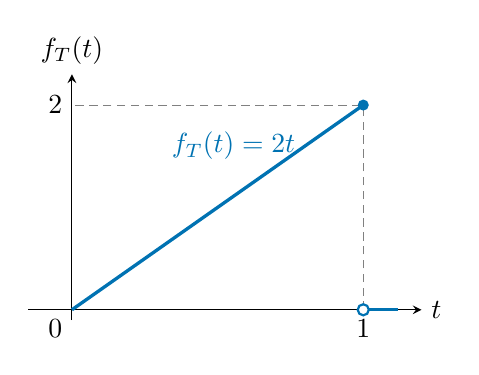
\begin{tikzpicture}[x=3.7cm,y=1.3cm,>=stealth]
\draw[->] (-.15,0)--(1.2,0) node[right] {$t$};
\draw[->] (0,-.1)--(0,2.3) node[above] {$f_T(t)$};
\draw[blue,very thick] (0,0)--(1,2);
\draw[blue,very thick] (1,0)--(1.12,0);
\draw[gray,densely dashed] (1,0)--(1,2)--(0,2);
\fill[blue] (1,2) circle[radius=2pt];
\draw[blue,fill=white,thick] (1,0) circle[radius=2pt];
\node[below left] at (0,0) {$0$};
\node[below] at (1,0) {$1$};
\node[left] at (0,2) {$2$};
\node[blue,left] at (.8,1.6) {$f_T(t)=2t$};
\end{tikzpicture}
\end{column}
\end{columns}
\vspace{.2cm}
The density is nonnegative and its total area is one; its integral gives accumulated probability.
\end{frame}

\begin{frame}{Solution 2: Probabilities are shaded areas (continued)}
\small
\answerpart{3}
\begin{columns}[T]
\begin{column}{.48\textwidth}
\centering
\textbf{Waiting at most half an hour}
\begin{center}
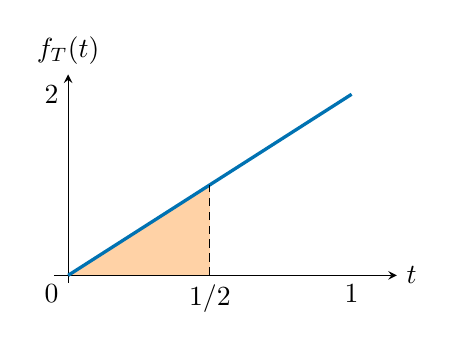
\begin{tikzpicture}[x=3.6cm,y=1.15cm,>=stealth]
\fill[orange!35] (0,0)--(.5,0)--(.5,1)--cycle;
\draw[->] (-.05,0)--(1.16,0) node[right] {$t$};
\draw[->] (0,-.08)--(0,2.22) node[above] {$f_T(t)$};
\draw[blue,very thick] (0,0)--(1,2);
\draw[densely dashed] (.5,0)--(.5,1);
\node[below left] at (0,0) {$0$};
\node[below] at (.5,0) {$1/2$};
\node[below] at (1,0) {$1$};
\node[left] at (0,2) {$2$};
\end{tikzpicture}
\end{center}
\[
\Pr(T\leq\tfrac12)=\int_0^{1/2}2t\,dt
=\left[t^2\right]_0^{1/2}=\boxed{\tfrac14}.
\]
\end{column}
\begin{column}{.48\textwidth}
\centering
\textbf{Waiting between 15 and 45 minutes}
\begin{center}
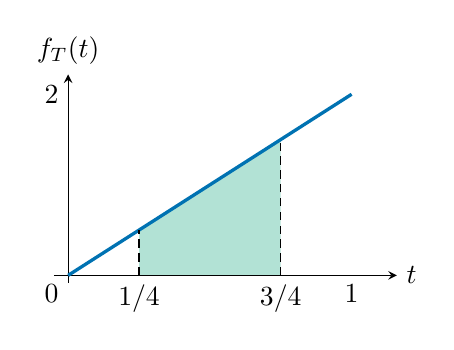
\begin{tikzpicture}[x=3.6cm,y=1.15cm,>=stealth]
\fill[green!30] (.25,0)--(.75,0)--(.75,1.5)--(.25,.5)--cycle;
\draw[->] (-.05,0)--(1.16,0) node[right] {$t$};
\draw[->] (0,-.08)--(0,2.22) node[above] {$f_T(t)$};
\draw[blue,very thick] (0,0)--(1,2);
\draw[densely dashed] (.25,0)--(.25,.5);
\draw[densely dashed] (.75,0)--(.75,1.5);
\node[below left] at (0,0) {$0$};
\node[below] at (.25,0) {$1/4$};
\node[below] at (.75,0) {$3/4$};
\node[below] at (1,0) {$1$};
\node[left] at (0,2) {$2$};
\end{tikzpicture}
\end{center}
\[
\Pr(\tfrac14<T\leq\tfrac34)=\frac9{16}-\frac1{16}=\boxed{\tfrac12}.
\]
\end{column}
\end{columns}
\vspace{.15cm}
\answerpart{4}$\Pr(T=3/4)=0$: a single point has zero area. The height $f_T(3/4)=3/2$ per hour is allowed; probabilities are integrals, not density heights.
\end{frame}
% SOLUTION 2 END
\fi

\begin{frame}{Problem 3: What are typical weekly earnings?}
Use the earnings distribution from Problem 1:
\begin{center}
\begin{tabular}{c|ccc}
$w$ (hundreds of euros) & 0 & 1 & 3 \\ \hline
$\Pr(W=w)$ & $1/2$ & $1/4$ & $1/4$
\end{tabular}
\end{center}
\begin{enumerate}
\setlength{\itemsep}{7pt}
\item Compute $\mu_W=\E(W)$ and $\E(W^2)$.
\item Calculate $\Var(W)$ from the weighted squared deviations. Check it using $\E(W^2)-[\E(W)]^2$.
\end{enumerate}
\end{frame}
\note{Solution to Problem 3. E(W)=0(.5)+1(.25)+3(.25)=1. E(W squared)=.25+2.25=2.5. The direct variance is .5(0-1) squared+.25(1-1) squared+.25(3-1) squared=.5+0+1=1.5. The shortcut is 2.5-1=1.5.}

\ifshowsolutions
% SOLUTION 3 START
\begin{frame}{Solution 3: Average earnings and variance}
\small
\answerpart{1}
\[
\E(W)=\tfrac12(0)+\tfrac14(1)+\tfrac14(3)=1,
\qquad \E(W^2)=\tfrac14(1)+\tfrac14(9)=\tfrac52.
\]
\answerpart{2}
\begin{columns}[T]
\begin{column}{.48\textwidth}
\textbf{Weighted squared deviations}
\begin{align*}
\Var(W)&=\tfrac12(0-1)^2+\tfrac14(1-1)^2\\
&\quad+\tfrac14(3-1)^2\\
&=\tfrac12+0+1=\boxed{\tfrac32}.
\end{align*}
\end{column}
\begin{column}{.48\textwidth}
\textbf{Second-moment shortcut}
\begin{align*}
\Var(W)&=\E(W^2)-[\E(W)]^2\\
&=\tfrac52-1^2=\boxed{\tfrac32}.
\end{align*}
\end{column}
\end{columns}
\end{frame}
% SOLUTION 3 END
\fi

\section{Two Variables}

\begin{frame}{Problem 4: Do participants find jobs more often?}
For a randomly selected student, let $D=1$ denote training participation and $H=1$ employment. The table gives joint probabilities from an observational population.
\jobtable
\begin{enumerate}
\setlength{\itemsep}{7pt}
\item Complete the marginal totals. Find $\Pr(D=1,H=1)$.
\item Calculate $\Pr(H=1\mid D=1)$, $\Pr(D=1\mid H=1)$, and $\Pr(H=1\mid D=0)$.
\item Find $\E(H\mid D=1)$ and $\E(H\mid D=0)$. Use iterated expectations to recover $\E(H)$.
\end{enumerate}
\end{frame}
\note{Solution to Problem 4. Row margins are .4 and .6; column margins are .6 and .4. Joint P(D=1,H=1)=.30. P(H=1|D=1)=.30/.40=.75; P(D=1|H=1)=.30/.60=.50; P(H=1|D=0)=.30/.60=.50. Because H is binary, conditional means equal employment probabilities. LIE gives .75(.40)+.50(.60)=.60, agreeing with the marginal mean. Reverse conditioning uses a different denominator.}

\ifshowsolutions
% SOLUTION 4 START
\begin{frame}{Solution 4: Participation, employment, and conditioning}
\small
\answerpart{1}
\begin{columns}[c]
\begin{column}{.39\textwidth}
\begin{center}
\begin{tabular}{c|cc|c}
 & $D=0$ & $D=1$ & Total \\ \hline
$H=0$ & .30 & .10 & .40 \\
$H=1$ & .30 & .30 & .60 \\ \hline
Total & .60 & .40 & 1
\end{tabular}
\end{center}
\[
\Pr(D=1,H=1)=.30.
\]
\end{column}
\begin{column}{.58\textwidth}
\answerpart{2}
\begin{align*}
\Pr(H=1\mid D=1)&=\frac{.30}{.40}=.75,\\
\Pr(D=1\mid H=1)&=\frac{.30}{.60}=.50,\\
\Pr(H=1\mid D=0)&=\frac{.30}{.60}=.50.
\end{align*}
\end{column}
\end{columns}
\answerpart{3}
Because $H$ is binary, $\E(H\mid D=d)=\Pr(H=1\mid D=d)$. Therefore
\begin{align*}
\E(H)&=\E[\E(H\mid D)]\\
&=.75\Pr(D=1)+.50\Pr(D=0)=.75(.40)+.50(.60)=\boxed{.60}.
\end{align*}
\end{frame}
% SOLUTION 4 END
\fi

\begin{frame}{Problem 5: What would independence look like?}
Before training begins, an independent lottery assigns $A=1$ with probability .40. Use the marginal distribution of $H$ from Problem 4. Lottery assignment is independent of $H$.
\begin{enumerate}
\setlength{\itemsep}{8pt}
\item Use independence to construct the full joint probability table of $(A,H)$, including marginal totals.
\item Calculate $\Pr(H=1\mid A=1)$, $\E(AH)$, and $\E(A)\E(H)$.
\end{enumerate}
\end{frame}
\note{Solution to Problem 5. The joint table has H=0 row (.24,.16) and H=1 row (.36,.24), in columns A=0,A=1. Column totals are .60,.40 and row totals .40,.60. Each cell is a product of margins. P(H=1|A=1)=.24/.40=.60. E(AH)=.24=.40(.60)=E(A)E(H).}

\ifshowsolutions
% SOLUTION 5 START
\begin{frame}{Solution 5: Independence before the programme}
\small
\answerpart{1}
\begin{columns}[c]
\begin{column}{.39\textwidth}
\begin{center}
\begin{tabular}{c|cc|c}
 & $A=0$ & $A=1$ & Total \\ \hline
$H=0$ & .24 & .16 & .40 \\
$H=1$ & .36 & .24 & .60 \\ \hline
Total & .60 & .40 & 1
\end{tabular}
\end{center}
\end{column}
\begin{column}{.58\textwidth}
Every cell factorizes:
\begin{align*}
\Pr(A=0,H=0)&=.60(.40)=.24,\\
\Pr(A=1,H=0)&=.40(.40)=.16,\\
\Pr(A=0,H=1)&=.60(.60)=.36,\\
\Pr(A=1,H=1)&=.40(.60)=.24.
\end{align*}
\end{column}
\end{columns}
\answerpart{2}
\[
\Pr(H=1\mid A=1)=\frac{.24}{.40}=.60=\Pr(H=1),
\qquad \E(AH)=.24=.40(.60)=\E(A)\E(H).
\]
\end{frame}
% SOLUTION 5 END
\fi

\begin{frame}{Problem 6: How strongly do training and jobs move together?}
Return to the observational population in Problem 4:
\jobtable
\begin{enumerate}
\setlength{\itemsep}{7pt}
\item Find $\E(D)$, $\E(H)$, $\Var(D)$, $\Var(H)$, and $\E(DH)$.
\item Calculate $\Cov(D,H)=\E(DH)-\E(D)\E(H)$. Interpret its sign.
\item Find $\Corr(D,H)$. Explain the role of standard deviations in this calculation.
\item Recode participation as $Q=100D$. Find $\Cov(Q,H)$ and $\Corr(Q,H)$. What happens to correlation if employment is replaced with unemployment $U=1-H$?
\end{enumerate}
\end{frame}
\note{Solution to Problem 6. E(D)=.4, E(H)=.6, and both variances equal .24, using p(1-p). E(DH)=.30. Covariance=.30-.4(.6)=.06, positive because participation and employment tend to move together. Correlation=.06/sqrt(.24 times .24)=.25. Dividing by standard deviations removes units. Cov(100D,H)=6; Corr(100D,H)=.25. For U=1-H, Cov(D,U)=-.06 and Corr(D,U)=-.25. These associations do not identify an effect of participation.}

\ifshowsolutions
% SOLUTION 6 START
\begin{frame}{Solution 6: Means, variances, and product moment}
\small
\answerpart{1}For any binary variable $B\in\{0,1\}$ with $p_B=\Pr(B=1)$,
\[
\E(B)=\sum_{b=0}^1 b\Pr(B=b)=p_B,\qquad
\Var(B)=\E(B^2)-[\E(B)]^2=p_B-p_B^2=p_B(1-p_B),
\]
using $B^2=B$. From the joint distribution in Problem 4,
\begin{align*}
\E(D)&=0(.60)+1(.40)=.40,
&\E(H)&=0(.40)+1(.60)=.60,\\
\Var(D)&=.40(1-.40)=.24,
&\Var(H)&=.60(1-.60)=.24.
\end{align*}
The product expectation is
\begin{align*}
\E(DH)&=\sum_{d=0}^1\sum_{h=0}^1 dh\Pr(D=d,H=h)\\
&=0(.30)+0(.10)+0(.30)+1(.30)=.30.
\end{align*}
Only the $(D,H)=(1,1)$ cell contributes, so $\E(DH)=\Pr(D=1,H=1)$.
\end{frame}

\begin{frame}{Solution 6: Covariance from the lecture definition}
\small
\answerpart{2}\textit{Lecture 1, ``Covariance''} defines covariance using deviations from the means. Let $\mu_D=\E(D)$ and $\mu_H=\E(H)$. Expanding that definition gives
\begin{align*}
\Cov(D,H)
&=\E[(D-\mu_D)(H-\mu_H)]\\
&=\E[DH-\mu_D H-\mu_H D+\mu_D\mu_H]\\
&=\E(DH)-\mu_D\E(H)-\mu_H\E(D)+\mu_D\mu_H\\
&=\E(DH)-\mu_D\mu_H\\
&=\E(DH)-\E(D)\E(H).
\end{align*}
The means are constants, so the cross terms reduce to the product of the means. Here,
\[
\Cov(D,H)=.30-(.40)(.60)=\boxed{.06}.
\]
Positive covariance indicates that participation and employment tend to move together.
\end{frame}

\begin{frame}{Solution 6: Correlation and recoding (continued)}
\small
\answerpart{3}
\[
\Corr(D,H)=\frac{.06}{\sqrt{.24}\sqrt{.24}}=\frac{.06}{.24}=\boxed{.25}.
\]
Dividing by standard deviations removes units and gives a scale-invariant measure of linear association.
\begin{block}{Recoding the variables}
\answerpart{4}
For $Q=100D$ and $U=1-H$,
\begin{align*}
\Cov(Q,H)&=100(.06)=6, &\Corr(Q,H)&=.25,\\
\Cov(D,U)&=-\Cov(D,H)=-.06, &\Corr(D,U)&=-.25.
\end{align*}
Positive scaling preserves correlation; reversing the employment indicator reverses its sign.
\end{block}
These associations alone do not identify a causal effect of training.
\end{frame}
% SOLUTION 6 END
\fi

\begin{frame}{Problem 7: Can zero correlation hide a relationship?}
A student's deviation from target work hours is $X\in\{-1,0,1\}$, with each value equally likely. The scheduling penalty index is $Z=X^2$.
\begin{enumerate}
\setlength{\itemsep}{8pt}
\item List the possible pairs $(X,Z)$ and their joint probabilities.
\item Calculate $\E(X)$, $\E(Z)$, $\Var(X)$, and $\Var(Z)$.
\item Find $\E(XZ)$, $\Cov(X,Z)$, and $\Corr(X,Z)$.
\item Compare $\Pr(Z=0\mid X=0)$ with $\Pr(Z=0)$. Are $X$ and $Z$ independent?
\item Explain why your answers about correlation and independence are compatible.
\end{enumerate}
\end{frame}
\note{Solution to Problem 7. The pairs are (-1,1),(0,0),(1,1), each with probability 1/3. E(X)=0, E(Z)=2/3. Var(X)=2/3 and Var(Z)=2/3-(2/3) squared=2/9. E(XZ)=E(X cubed)=0; covariance and correlation are zero because both variances are positive. P(Z=0|X=0)=1 whereas P(Z=0)=1/3, so independence fails. Z is completely determined by X but the relationship is nonlinear and symmetric around zero. Independence implies zero covariance when the moments exist; the converse fails.}

\ifshowsolutions
% SOLUTION 7 START
\begin{frame}{Solution 7: Zero correlation can hide dependence}
\small
\answerpart{1}
\begin{columns}[T]
\begin{column}{.43\textwidth}
\begin{center}
\begin{tabular}{cc|c}
$X$ & $Z=X^2$ & Probability \\ \hline
$-1$ & 1 & $1/3$ \\
0 & 0 & $1/3$ \\
1 & 1 & $1/3$
\end{tabular}
\end{center}
\answerpart{2}
\begin{align*}
\E(X)&=0,&\E(Z)&=\frac23,\\
\Var(X)&=\frac23,&\Var(Z)&=\frac23-\left(\frac23\right)^2=\frac29.
\end{align*}
\end{column}
\begin{column}{.54\textwidth}
\answerpart{3}
\begin{align*}
\E(XZ)&=\frac{-1+0+1}{3}=0,\\
\Cov(X,Z)&=0-0\left(\frac23\right)=0,\\
\Corr(X,Z)&=\frac{0}{\sqrt{2/3}\sqrt{2/9}}=0.
\end{align*}
Yet conditioning changes the distribution:
\answerpart{4}
\[
\Pr(Z=0\mid X=0)=1\ne\frac13=\Pr(Z=0).
\]
\end{column}
\end{columns}
\vspace{.15cm}
\answerpart{5}
\begin{exampleblock}{Interpretation}
$X$ and $Z$ are dependent: $X$ determines $Z$ exactly. Correlation measures linear association and can be zero for a nonlinear relationship.
\end{exampleblock}
\end{frame}
% SOLUTION 7 END
\fi

\begin{frame}{Problem 8: How risky is a two-part support payment?}
Use the observational $(D,H)$ distribution from Problem 4. You found
\[
\E(D)=.40,\quad \E(H)=.60,\quad
\Var(D)=\Var(H)=.24,\quad\Cov(D,H)=.06.
\]
The university pays 100 euros for participating in training and 200 euros for being employed. Total support is $S=100D+200H$.
\begin{enumerate}
\setlength{\itemsep}{7pt}
\item Compute $\E(S)$, $\Var(S)$, and its standard deviation. Include the covariance term.
\item How much would the variance be understated if covariance were incorrectly set to zero?
\end{enumerate}
\end{frame}
\note{Solution to Problem 8. E(S)=100(.4)+200(.6)=160 euros. Var(S)=100 squared(.24)+200 squared(.24)+2(100)(200)(.06)=2400+9600+2400=14400 euros squared. SD=120 euros. Ignoring covariance gives 12000 and understates the variance by 2400 euros squared. Dependence affects the risk of a sum.}

\ifshowsolutions
% SOLUTION 8 START
\begin{frame}{Solution 8: The risk of a two-part support payment}
\small
\answerpart{1}
For $S=100D+200H$, expected support is
\[
\E(S)=100(.40)+200(.60)=160\text{ euros}.
\]
\begin{align*}
\Var(S)&=100^2\Var(D)+200^2\Var(H)+2(100)(200)\Cov(D,H)\\
&=2{,}400+9{,}600+2{,}400=14{,}400\text{ euros}^2,\\
\operatorname{SD}(S)&=\sqrt{14{,}400}=120\text{ euros}.
\end{align*}
\answerpart{2}Omitting covariance gives $12{,}000$ euros$^2$, understating variance by $2{,}400$ euros$^2$.
\end{frame}
% SOLUTION 8 END
\fi

\section{Sampling}

\begin{frame}{Problem 9: What can two employment responses tell us?}
Employment indicators $H_1$ and $H_2$ are independent draws from a population with $\Pr(H_i=1)=.60$. Define
\[
\overline H=\frac{H_1+H_2}{2}.
\]
\begin{enumerate}
\setlength{\itemsep}{8pt}
\item List the four ordered samples $(H_1,H_2)$ and their probabilities.
\item Construct the exact sampling distribution of $\overline H$.
\item Calculate $\E(\overline H)$ and $\Var(\overline H)$ directly from that distribution.
\item Check your answers using $\E(\overline H)=\mu_H$ and $\Var(\overline H)=\sigma_H^2/n$.
\end{enumerate}
\end{frame}
\note{Solution to Problem 9. Ordered samples (0,0),(0,1),(1,0),(1,1) have probabilities .16,.24,.24,.36. Sample means 0,.5,1 have probabilities .16,.48,.36. E(Hbar)=.5(.48)+1(.36)=.6. E(Hbar squared)=.25(.48)+.36=.48, and variance=.48-.36=.12. Population variance=.6(.4)=.24, so .24/2=.12.}

\ifshowsolutions
% SOLUTION 9 START
\begin{frame}{Solution 9: The exact sampling distribution}
\small
\answerpart{1}Independence gives the probability of each ordered pair as a product:
\begin{columns}[T]
\begin{column}{.49\textwidth}
\centering
\begin{tabular}{ccc}
\toprule
$(H_1,H_2)$ & Probability & $\overline H$ \\
\midrule
$(0,0)$ & $.4\times.4=.16$ & $0$ \\
$(0,1)$ & $.4\times.6=.24$ & $.5$ \\
$(1,0)$ & $.6\times.4=.24$ & $.5$ \\
$(1,1)$ & $.6\times.6=.36$ & $1$ \\
\bottomrule
\end{tabular}
\end{column}
\begin{column}{.47\textwidth}
\centering
\answerpart{2}
\textbf{Collect equal values of the average:}\par\vspace{4pt}
\begin{tabular}{cc}
\toprule
$h$ & $\Pr(\overline H=h)$ \\
\midrule
$0$ & $.16$ \\
$.5$ & $.24+.24=.48$ \\
$1$ & $.36$ \\
\bottomrule
\end{tabular}
\end{column}
\end{columns}
\vspace{.1cm}
\answerpart{3}
\[
\begin{aligned}
\E(\overline H)&=0(.16)+.5(.48)+1(.36)=.60,\\
\E(\overline H^2)&=0^2(.16)+.5^2(.48)+1^2(.36)=.48,\\
\Var(\overline H)&=.48-(.60)^2=.12.
\end{aligned}
\]
\answerpart{4}The i.i.d. formula confirms $\E(\overline H)=.60=\mu_H$ and $\Var(\overline H)=.12=\sigma_H^2/2=.60(.40)/2$.
\end{frame}
% SOLUTION 9 END
\fi

\begin{frame}{Problem 10: How precise is a survey's average wage?}
For this problem and Problem 11, model hourly wages $Y_1,\ldots,Y_n$ as i.i.d. draws with population mean $\mu_Y=15$ euros and standard deviation $\sigma_Y=6$ euros.
\begin{enumerate}
\setlength{\itemsep}{8pt}
\item Derive $\E(\overline Y)$ and $\Var(\overline Y)$. Identify where independence is used.
\item Compute the variance and standard deviation of $\overline Y$ for $n=25$ and $n=100$.
\item Does quadrupling the sample size divide the standard deviation by four?
\item How large must $n$ be for the standard deviation of $\overline Y$ to be at most .50 euros?
\item If students' wages are positively correlated, what missing terms would make the i.i.d. variance formula too small?
\end{enumerate}
\end{frame}
\note{Solution to Problem 10. E(Ybar)=mu=15. Var(Ybar)=n inverse squared times [sum of individual variances plus sum over all distinct i,j of Cov(Yi,Yj)]. Under independence the covariance terms vanish, yielding 36/n. At n=25 variance=1.44 euros squared and SD=1.20 euros; at n=100 variance=.36 and SD=.60. Quadrupling n halves the SD. Solve 6/sqrt(n)<=.50 to obtain n>=144. Positive cross-observation covariances raise the variance; they cannot be omitted merely because each observation has the same marginal distribution.}

\ifshowsolutions
% SOLUTION 10 START
\begin{frame}{Solution 10: Sample size and earnings precision}
\small
\answerpart{1}
\[
\E(\overline Y)=\frac1n\sum_{i=1}^n\E(Y_i)=15,
\qquad
\begin{aligned}
\Var(\overline Y)
&=\frac1{n^2}\left[\sum_{i=1}^n\Var(Y_i)+\sum_{i\ne j}\Cov(Y_i,Y_j)\right]\\
&=\frac{36n+0}{n^2}=\frac{36}{n}.
\end{aligned}
\]
Independence makes the cross-observation covariances zero. Therefore $\operatorname{SD}(\overline Y)=6/\sqrt n$.
\begin{center}
\answerpart{2}
\begin{tabular}{ccc}
\toprule
Sample size & $\Var(\overline Y)$ (euros squared) & $\operatorname{SD}(\overline Y)$ (euros) \\
\midrule
$25$ & $36/25=1.44$ & $1.20$ \\
$100$ & $36/100=.36$ & $.60$ \\
\bottomrule
\end{tabular}
\end{center}
\begin{itemize}
\setlength{\itemsep}{5pt}
\item \answerpart{3}Quadrupling $n$ \textbf{halves} the SD: $6/\sqrt{4n}=\tfrac12(6/\sqrt n)$.
\item \answerpart{4}For SD at most $.50$: $6/\sqrt n\leq .50\iff\sqrt n\geq12\iff n\geq144$.
\item \answerpart{5}Positive covariances add $n^{-2}\sum_{i\ne j}\Cov(Y_i,Y_j)$ to the variance. Omitting them understates uncertainty.
\end{itemize}
\end{frame}
% SOLUTION 10 END
\fi





\begin{frame}{Problem 11: Is an unusually high survey mean surprising?}
Hourly wages are i.i.d., with $\mu_Y=15$ euros and $\sigma_Y=6$ euros. The population distribution is right skewed with finite variance. A survey samples $n=100$ students. Assume the CLT approximation is adequate at this sample size.
\begin{enumerate}
\setlength{\itemsep}{8pt}
\item Use the central limit theorem to approximate the distribution of $\overline Y$. State whether the second normal parameter is a variance or a standard deviation.
\item Standardize and approximate $\Pr(\overline Y>16.20)$.
\item Approximate $\Pr(13.80\leq\overline Y\leq16.20)$.
\item Would the normal approximation be exact for this population? What changes if the population itself is normal? Is the approximation automatically reliable at $n=4$?
\end{enumerate}
\vspace{.1cm}
Use $\Phi(2)=.9772$ and $\Phi(-2)=.0228$, where $\Phi$ is the standard normal c.d.f.
\end{frame}
\note{Solution to Problem 11. Ybar is approximately normal with mean 15 and variance 36/100=.36; the SD is .6. At 16.2 the standardized value is (16.2-15)/.6=2. Thus P(Ybar>16.2) is approximately 1-.9772=.0228. The lower endpoint gives -2, so the central interval probability is approximately .9772-.0228=.9544. For the right-skewed population this is a CLT approximation, not an exact finite-sample distribution. Finite variance establishes the asymptotic CLT but supplies no universal guarantee at n=100; strong skewness or rare outliers may slow convergence. A normal population gives an exact normal sample mean for every n. At n=4 reliability must be assessed rather than assumed. The CLT describes the standardized distribution; the LLN describes concentration around the mean.}

\ifshowsolutions
% SOLUTION 11 START
\begin{frame}{Solution 11: A high average under the CLT}
\small
\answerpart{1}
At $n=100$, the assumed CLT approximation gives
\[
\overline Y\ \overset{a}{\sim}\ \mathcal N\left(15,\frac{36}{100}\right)
=\mathcal N(15,.36).
\]
\[
\operatorname{SD}(\overline Y)=\sqrt{\Var(\overline Y)}=\sqrt{.36}=.60\text{ euros}.
\]
\[
Z=\frac{\overline Y-15}{.60}\ \overset{a}{\sim}\ \mathcal N(0,1).
\]
The second normal parameter is the variance; its square root is the standard deviation.
\par\answerpart{2}
\[
\Pr(\overline Y>16.20)
\approx\Pr\left(Z>\frac{16.20-15}{.60}\right)
=1-\Phi(2)=.0228.
\]
\answerpart{3}
\[
\Pr(13.80\leq\overline Y\leq16.20)
\approx\Pr(-2\leq Z\leq2)=\Phi(2)-\Phi(-2)=.9544.
\]
\begin{itemize}
\setlength{\itemsep}{6pt}
\item \answerpart{4}For the right-skewed population these are approximate probabilities; if wages themselves are normal, the sample mean is \emph{exactly} normal at every $n$. Finite variance does not guarantee an accurate approximation at $n=4$; skewness and rare outliers affect finite-sample accuracy.
\end{itemize}
\end{frame}
% SOLUTION 11 END
\fi

\section{Estimation}

\begin{frame}{Problem 12: Which wage estimator should we use?}
Let $Y_1,\ldots,Y_n$ be i.i.d. with unknown mean $\mu_Y$ and variance $36$. Consider
\[
A_n=\overline Y_n,\qquad B_n=Y_1,\qquad
C_n=\overline Y_n+1,\qquad T_n=\frac{n-1}{n}\overline Y_n.
\]
\begin{enumerate}
\setlength{\itemsep}{7pt}
\item For each rule, find its expectation, bias, and variance. Which are unbiased for all $\mu_Y$?
\item Which rules are consistent for $\mu_Y$? Explain what happens as $n\to\infty$.
\item At $n=100$, which unbiased rule is more efficient? Does a smaller variance alone make a biased rule preferable?
\item For the observed wages $(9,12,15,18,21)$, compute the four estimates with $n=5$. Distinguish each estimator from its realized estimate.
\end{enumerate}
\end{frame}
\note{Solution to Problem 12. A has expectation mu, bias 0, variance 36/n, and is consistent. B has expectation mu, bias 0, variance 36, and is not consistent for a nondegenerate population: adding observations does not change Y1. C has expectation mu+1, bias 1, variance 36/n, and converges to mu+1, so it is inconsistent. T has expectation (1-1/n)mu, bias -mu/n, variance (1-1/n) squared times 36/n, and is consistent; it is not unbiased for all mu. At n=100, A has variance .36 versus B's 36 and is more efficient among these unbiased rules. T has slightly smaller variance than A but is biased in general; variance alone is not an accuracy ranking across biased and unbiased estimators. With the five wages, ybar=15 and estimates A=15, B=9, C=16, T=12. The estimator is the formula before observing data; the estimate is the resulting number.}

\ifshowsolutions
% SOLUTION 12 START
\begin{frame}{Solution 12: Bias and consistency of four rules}
\small
\answerpart{1}
Let $a_n=(n-1)/n$. Linearity of expectation and $\Var(cX)=c^2\Var(X)$ give:
\begin{center}
\renewcommand{\arraystretch}{1.45}
\begin{tabular}{lccc}
\toprule
Estimator & Expectation & Bias for $\mu_Y$ & Variance \\
\midrule
$A_n=\overline Y_n$ & $\mu_Y$ & $0$ & $36/n$ \\
$B_n=Y_1$ & $\mu_Y$ & $0$ & $36$ \\
$C_n=\overline Y_n+1$ & $\mu_Y+1$ & $1$ & $36/n$ \\
$T_n=a_n\overline Y_n$ & $a_n\mu_Y$ & $-\mu_Y/n$ & $a_n^2\,36/n$ \\
\bottomrule
\end{tabular}
\end{center}
Thus \textbf{$A_n$ and $B_n$ are unbiased for every $\mu_Y$}.
\answerpart{2}
\begin{itemize}
\setlength{\itemsep}{6pt}
\item $A_n\xrightarrow{p}\mu_Y$ by the LLN: it is consistent.
\item $B_n=Y_1$ retains the same nondegenerate distribution as $n$ grows: it is inconsistent.
\item $C_n\xrightarrow{p}\mu_Y+1$: it is inconsistent for $\mu_Y$.
\item $a_n\to1$ and $\overline Y_n\xrightarrow{p}\mu_Y$, so $T_n\xrightarrow{p}\mu_Y$: it is consistent, although generally biased at finite $n$.
\end{itemize}
\end{frame}

\begin{frame}{Solution 12: Precision and realized estimates (continued)}
\small
\answerpart{3}\textbf{At $n=100$: compare the unbiased rules.}
\[
\Var(A_{100})=\frac{36}{100}=.36
\quad<\quad
\Var(B_{100})=36.
\]
The sample mean is more efficient than the first observation among these unbiased rules. Shrinkage reduces variance but introduces bias:
\[
\Var(T_{100})=.99^2(.36)=.352836,
\qquad
\E(T_{100})-\mu_Y=-.01\mu_Y.
\]
A smaller variance alone does not establish that a biased estimator is more accurate.
\vspace{.2cm}

\answerpart{4}\textbf{After observing $(9,12,15,18,21)$, use $n=5$:}
\[
\overline y=\frac{9+12+15+18+21}{5}=15,
\qquad
\begin{array}{c|cccc}
\text{rule} & A_5 & B_5 & C_5 & T_5\\ \hline
\text{estimate} & 15 & 9 & 16 & \frac45(15)=12
\end{array}
\]
An \emph{estimator} is the sample-based rule, random before observation; an \emph{estimate} is the numerical value produced by the observed sample.
\end{frame}
% SOLUTION 12 END
\fi

\begin{frame}{Problem 13: Why give every wage the same weight?}
Four i.i.d. wages have mean $\mu_Y$ and variance $36$. Normality is \emph{not} assumed. Compare
\[
M=\frac{Y_1+Y_2+Y_3+Y_4}{4},\qquad
L=\frac12Y_1+\frac16(Y_2+Y_3+Y_4).
\]
\begin{enumerate}
\setlength{\itemsep}{7pt}
\item Show that both estimators are linear and unbiased. Compare their variances.
\item For fixed weights, when is $\widehat\mu=\sum_{i=1}^n w_iY_i$ unbiased for every $\mu_Y$? Derive its variance under i.i.d. sampling.
\item Under the unbiasedness restriction, use
\[
\sum_{i=1}^n(w_i-1/n)^2=\sum_{i=1}^n w_i^2-1/n\geq0
\]
to find the minimum possible variance and the weights attaining it.
\item Explain each word in ``Best Linear Unbiased Estimator'' for the sample mean.
\end{enumerate}
\end{frame}
\note{Solution to Problem 13. Both fixed-weight sums have weights adding to 1 and expectation mu. Var(M)=36/4=9 euros squared. Var(L)=36[(1/2) squared+3(1/6) squared]=36(1/3)=12 euros squared. In general expectation is mu times sum(wi); unbiasedness for every mu requires sum(wi)=1. Independence and common variance give Var(muhat)=36 sum(wi squared). The displayed nonnegative sum implies sum(wi squared)>=1/n, with equality iff every wi=1/n. Thus the minimum variance in this class is 36/n, achieved by the sample mean. Best means smallest variance within the linear unbiased class; linear means a fixed weighted sum of the observations; unbiased means expected value equals the target. This result does not require normality and makes no unrestricted claim about all nonlinear estimators.}

\ifshowsolutions
% SOLUTION 13 START
\begin{frame}{Solution 13: Comparing two wage averages}
\small
\answerpart{1}
Both rules are fixed weighted sums, and both sets of weights sum to one:
\[
\E(M)=\frac14(4\mu_Y)=\mu_Y,
\qquad
\E(L)=\left(\frac12+3\cdot\frac16\right)\mu_Y=\mu_Y.
\]
Independence removes covariance terms, so
\[
\begin{aligned}
\Var(M)&=36\left[4\left(\frac14\right)^2\right]=9,\\[3pt]
\Var(L)&=36\left[\left(\frac12\right)^2+3\left(\frac16\right)^2\right]=12.
\end{aligned}
\]
Thus $M$ is more efficient than $L$ among these two unbiased estimators.
\vspace{.15cm}

\answerpart{2}For any fixed weights $w_1,\ldots,w_n$ under the stated i.i.d. model,
\[
\E\left(\sum_{i=1}^n w_iY_i\right)=\mu_Y\sum_{i=1}^n w_i,
\qquad
\Var\left(\sum_{i=1}^n w_iY_i\right)=36\sum_{i=1}^n w_i^2.
\]
Unbiasedness for \emph{every} $\mu_Y$ requires $\sum_{i=1}^n w_i=1$.
\end{frame}

\begin{frame}{Solution 13: Why equal weights are BLUE (continued)}
\small
\answerpart{3}Impose the unbiasedness restriction $\sum_{i=1}^n w_i=1$. Then
\[
\begin{aligned}
0\leq\sum_{i=1}^n\left(w_i-\frac1n\right)^2
&=\sum_{i=1}^n w_i^2-\frac2n\sum_{i=1}^n w_i+\frac{n}{n^2}\\
&=\sum_{i=1}^n w_i^2-\frac1n.
\end{aligned}
\]
Consequently,
\[
\Var\left(\sum_{i=1}^n w_iY_i\right)=36\sum_{i=1}^n w_i^2
\ \geq\ \frac{36}{n},
\]
with equality precisely when $w_i=1/n$ for every $i$. The attaining estimator is $\overline Y$.
\begin{itemize}
\setlength{\itemsep}{4pt}
\item \answerpart{4}\textbf{BLUE} means Best Linear Unbiased Estimator: best is smallest variance within the linear unbiased class, linear is a fixed weighted sum, and unbiased means the expectation equals the population mean.
\end{itemize}
Normality is unnecessary; i.i.d. sampling supplies the common mean, variance, and zero covariances used here.
\end{frame}
% SOLUTION 13 END
\fi

\end{document}
